\section{Realisation}
\label{sec:realisation} 
\begin{wrapfigure}[12]{r}{.40\textwidth}
  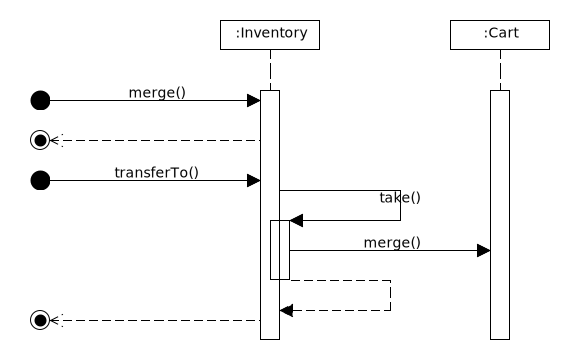
\includegraphics[width=.4\textwidth]{figures/fillInventorySellProduct_seqd}
  \caption{\label{seq:mergandtransfer}Fill the inventory (merge), then
    put a product from inventory into a cart.}
\end{wrapfigure}%
In figure~\ref{seq:mergandtransfer} you see a simplified model of the most
important business use case.
%
The application provides two implementations of the interface 
\Code{ProductContainer}:
\begin{enumerate*}
\item \Code{IMProductContainer} which is an in memory implementation.
\item \Code{PGDBProductContainer} which uses a database (in particular
  postgresql) as the persistence service.
\end{enumerate*}

See the class diagram figure~\ref{fig:classdiagram} for details in
relations.

In this exam you will have to test and implement some of the methods.
The test names and documentation should give you hints on what to
test. After you have written the tests, you can implement the methods.
\clearpage
\subsection{Persistence implementation}
\begin{wrapfigure}[18]{r}{.45\textwidth}\vspace{-2\baselineskip}  
  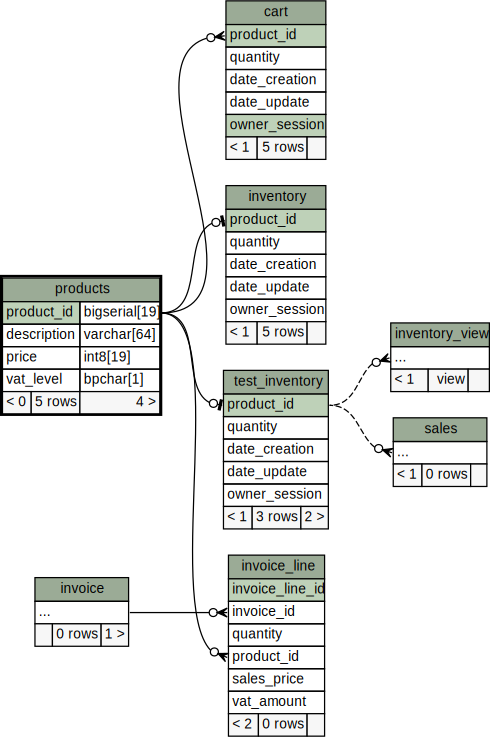
\includegraphics[width=.45\textwidth]{figures/products_implied2degrees.pdf}%\vspace{-2\baselineskip}  
  \caption{\label{dbschema}Simplified database schema}
\end{wrapfigure}%
In the realisation of the persistence version 
(\Code{PGDBProductContainer}) of the product 
container, the responsibility of some of the constraints
(e.g. quantity of a product must be non-negative) can be delegated to
the database. When such a constraint is violated, the database layer
will throw an exception, which is wrapped into a \Code{java.lang.RunException} 
but should be caught, inspected (unwrapped with \Code{Exception.getCause()} 
and dealt with in a business appropriate way. 
The database schema can be found in figure~\ref{dbschema}, 
but is also available on line during the exam in a more detailed form.
Note that the \Code{owner\_session} column identifies the cart, in case you
wonder why there is no \texttt{class\_id} column.

\subsection{The Façade between business and web}
In the design you find a Façade class, which provides one entry point to the
whole business model. In the class diagram you can find it too to see
what methods are provided by the webshopModel project to the webshop project.


\begin{sidewaysfigure}
  % \begin{figure}
  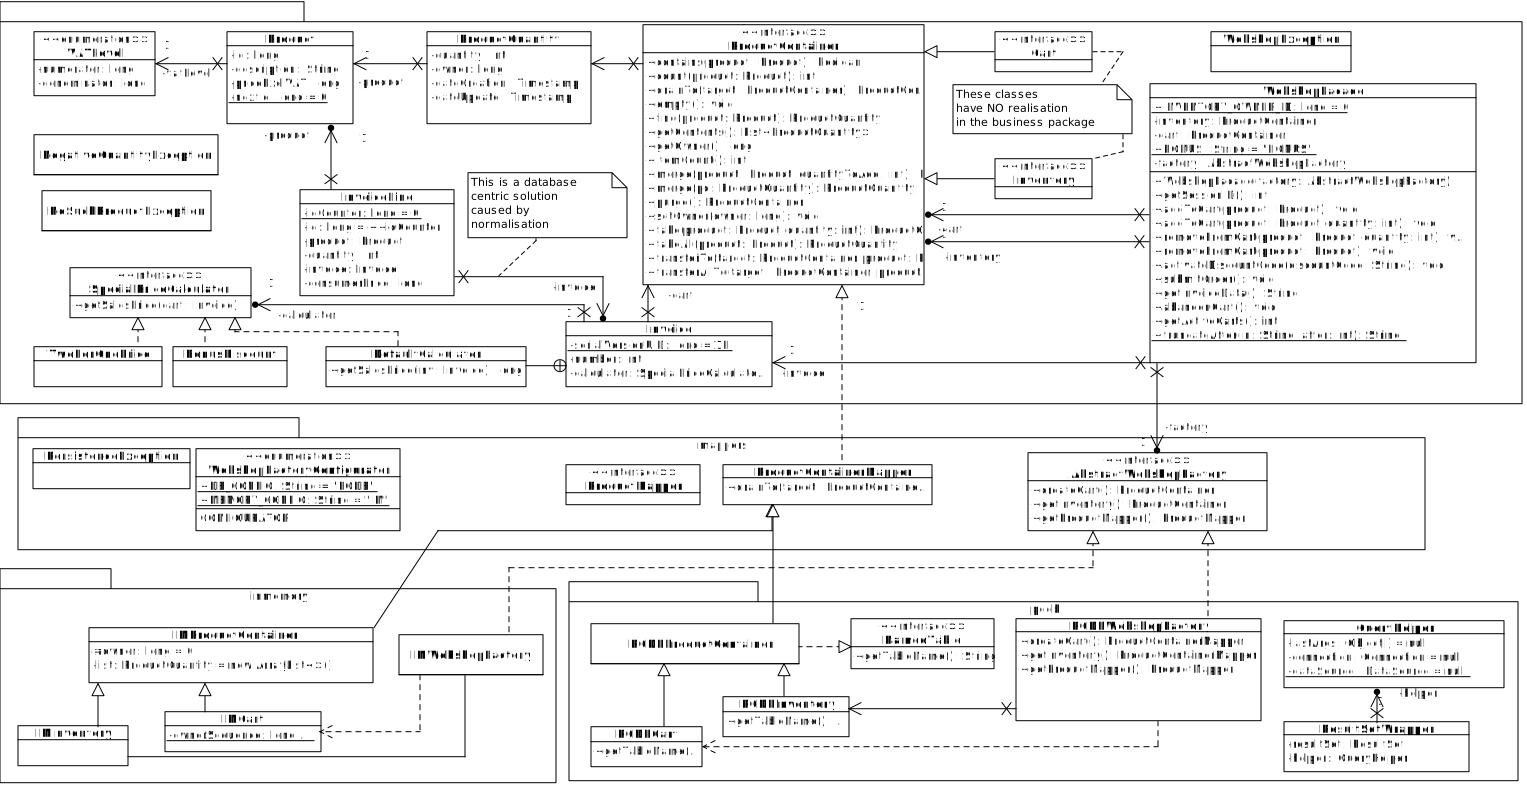
\includegraphics[width=\textwidth]{figures/webshop2015}
  \caption{\label{fig:classdiagram}Class diagram of the important types in the  business and
    persistence packages}
  % \end{figure}
\end{sidewaysfigure}

\vspace{5\baselineskip}

